%%%%%%%%%%%%%%%%%%%%%%%%%%%%%%%%%%%%%%%%%
% Stylish Article
% LaTeX Template
% Version 2.2 (2020-10-22)
%
% This template has been downloaded from:
% http://www.LaTeXTemplates.com
%
% Original author:
% Mathias Legrand (legrand.mathias@gmail.com) 
% With extensive modifications by:
% Vel (vel@latextemplates.com)
%
% License:
% CC BY-NC-SA 3.0 (http://creativecommons.org/licenses/by-nc-sa/3.0/)
%
%%%%%%%%%%%%%%%%%%%%%%%%%%%%%%%%%%%%%%%%%

%----------------------------------------------------------------------------------------
%	PACKAGES AND OTHER DOCUMENT CONFIGURATIONS
%----------------------------------------------------------------------------------------

\documentclass[fleqn,10pt]{SelfArx} % Document font size and equations flushed left

\usepackage[english]{babel} % Specify a different language here - english by default

\usepackage{lipsum} % Required to insert dummy text. To be removed otherwise
\usepackage{subcaption}
\captionsetup{compatibility=false}
%----------------------------------------------------------------------------------------
%	COLUMNS
%----------------------------------------------------------------------------------------

\setlength{\columnsep}{0.55cm} % Distance between the two columns of text
\setlength{\fboxrule}{0.75pt} % Width of the border around the abstract

%----------------------------------------------------------------------------------------
%	COLORS
%----------------------------------------------------------------------------------------

\definecolor{color1}{RGB}{0,0,90} % Color of the article title and sections
\definecolor{color2}{RGB}{0,20,20} % Color of the boxes behind the abstract and headings

%----------------------------------------------------------------------------------------
%	HYPERLINKS
%----------------------------------------------------------------------------------------

\usepackage{hyperref} % Required for hyperlinks

\hypersetup{
	hidelinks,
	colorlinks,
	breaklinks=true,
	urlcolor=color2,
	citecolor=color1,
	linkcolor=color1,
	bookmarksopen=false,
	pdftitle={Title},
	pdfauthor={Author},
}

%----------------------------------------------------------------------------------------
%	ARTICLE INFORMATION
%----------------------------------------------------------------------------------------

\JournalInfo{Anthony Sander} % Journal information
\Archive{Class Project} % Additional notes (e.g. copyright, DOI, review/research article)

\PaperTitle{AI TODO Personal Assistant} % Article title

\Authors{Basma Ashour  \textsuperscript{}, Saloni Vora\textsuperscript{}} % Authors
\affiliation{\textsuperscript{1}\textit{MIU, Computer Science}} % Author affiliation

\Keywords{Torch --- Wav2Vec --- NLP --- WakeWord} % Keywords - if you don't want any simply remove all the text between the curly brackets
\newcommand{\keywordname}{Keywords} % Defines the keywords heading name

%----------------------------------------------------------------------------------------
%	ABSTRACT
%----------------------------------------------------------------------------------------

\Abstract{In this paper we are gonna discuss how we build a speech recognition system with the wake word to detect what the user is saying and based on that we can add a new To-Do or remove a To-Do, the input is a record voice and the output is add/remove or todo or do nothing if it couldn't detect the speech or the user gave a command which is not add/remove}

%----------------------------------------------------------------------------------------

\begin{document}

\maketitle % Output the title and abstract box

\tableofcontents % Output the contents section

\thispagestyle{empty} % Removes page numbering from the first page

%----------------------------------------------------------------------------------------
%	ARTICLE CONTENTS
%----------------------------------------------------------------------------------------

\section*{Introduction} % The \section*{} command stops section numbering

\addcontentsline{toc}{section}{Introduction} % Adds this section to the table of contents

We First implemented the wake word using: Bidirectional LSTM(Long Short term Memory) \\
Then after the model is active due to the wake word we implemented the speech recognition using Wav2Vec2 model \\
Then build the Api to process the data that has been recognized from the wav2vec \\
Then we showed the result in the UI

%------------------------------------------------


%------------------------------------------------

\section{Wake Word Detection}

 

This problem is to wake up a system when a specific word or specific sequence of words are used. This is to wake up a Voice Assistant system to listen to the rest of the commands and take action on them. \\
The approach used to solve this problem is classification. We classify the data in 0 and 1 to identify if the wake word was spoken or not. 0 indicates the use of non-wake word and 1 indicates the use of wake word. \\ \\

 

1. Data Collection:  \\
    a. Wake word data collection : To collect the wake word data we have recorded the wake word 100 times using a script. \\
    b. Noise data collection : To collect the non wake word data/ noise data we recorded a 10 min audio to collect the noisy data around. \\ \\

 

2. Data Preprocessing: \\
    a. As the wake words sample is less in proportion than the non-wake word samples, we have upsampled teh data (multiplied teh occurance by 10) to increase teh proportion to increase teh accuracy of the system. \\
    b. Now since the noisy recording is just one sample we split it into chunks so that we get more recordings for training the system. \\
    c. Finally after performing both the above actions, we use teh combination of these files and create training and testing datasets which contain the .wav files and their key (0 or 1). \\ \\

 

4. Model: \\
    We have used a sequence to sequence model to resolve this problem. And the type used is a bidirectional LSTM(Long Short term Memory) model for our audio samples, with Normalization used as Layer Normalization and since our problem is a classification problem, we have used a liner classification to finally classify the result that we are predicting,
 \\ \\
 

5. Training: \\
    To train the model we need to get the sequence of numbers against the audio samples that we have used and to do the same we have used the 
    MFCC(Mel scale is a scale that relates the perceived frequency of a tone to the actual measured frequency.) technique. This technique transforms the audio data in the sequence of its frequency(numbers), now this data set can be further trained. \\ \\

 

7. Final Prediction: \\
    We have created threads in the main loop, where each thread runs for two seconds to listen to the audio and identify if the wake word was spoken or not. \\ \\

 

Currently due to lack of resources we have taken minimal data set(10 mins of noisy data and 200 wake word samples of 2 seconds each), and trained the system for 20 epochs only(due to which the model seems to be overfitting) and based on that following are the results :

\begin{figure}[h!]
  \centering
  \begin{subfigure}[b]{0.9\linewidth}
    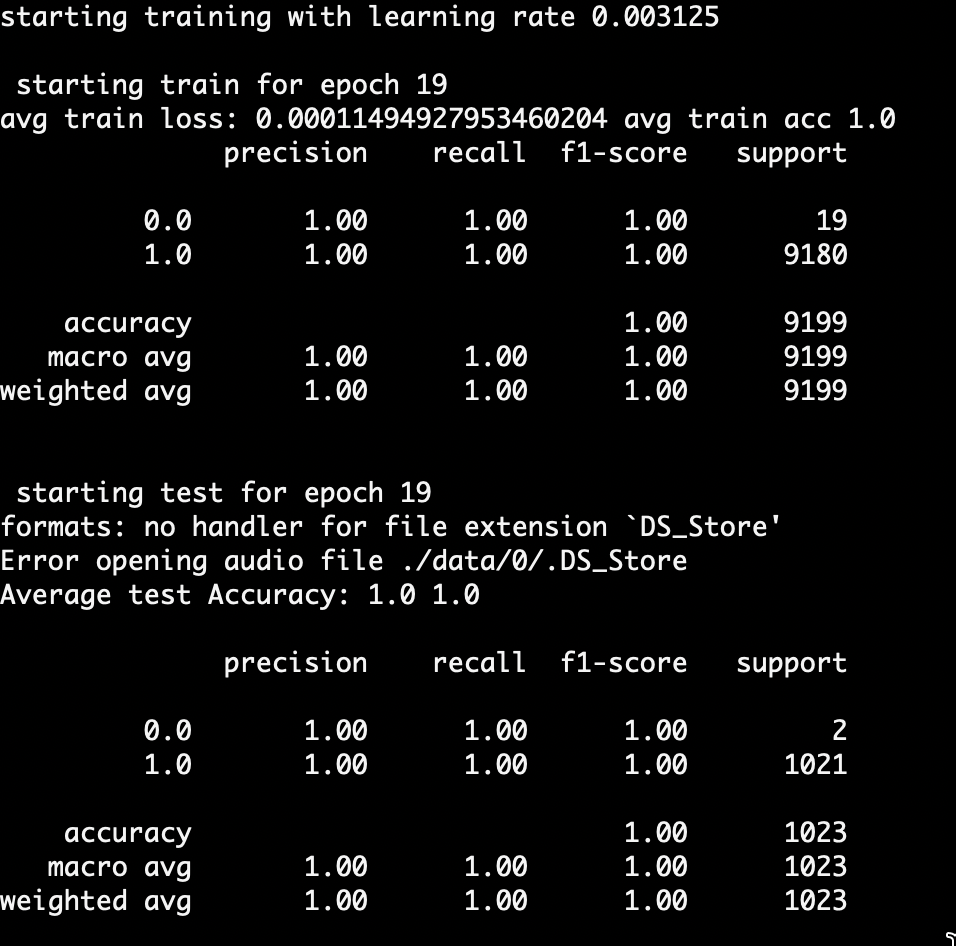
\includegraphics[width=\linewidth]{1.png}
    \caption{Accuracy1.}
  \end{subfigure}
  \begin{subfigure}[b]{0.9\linewidth}
    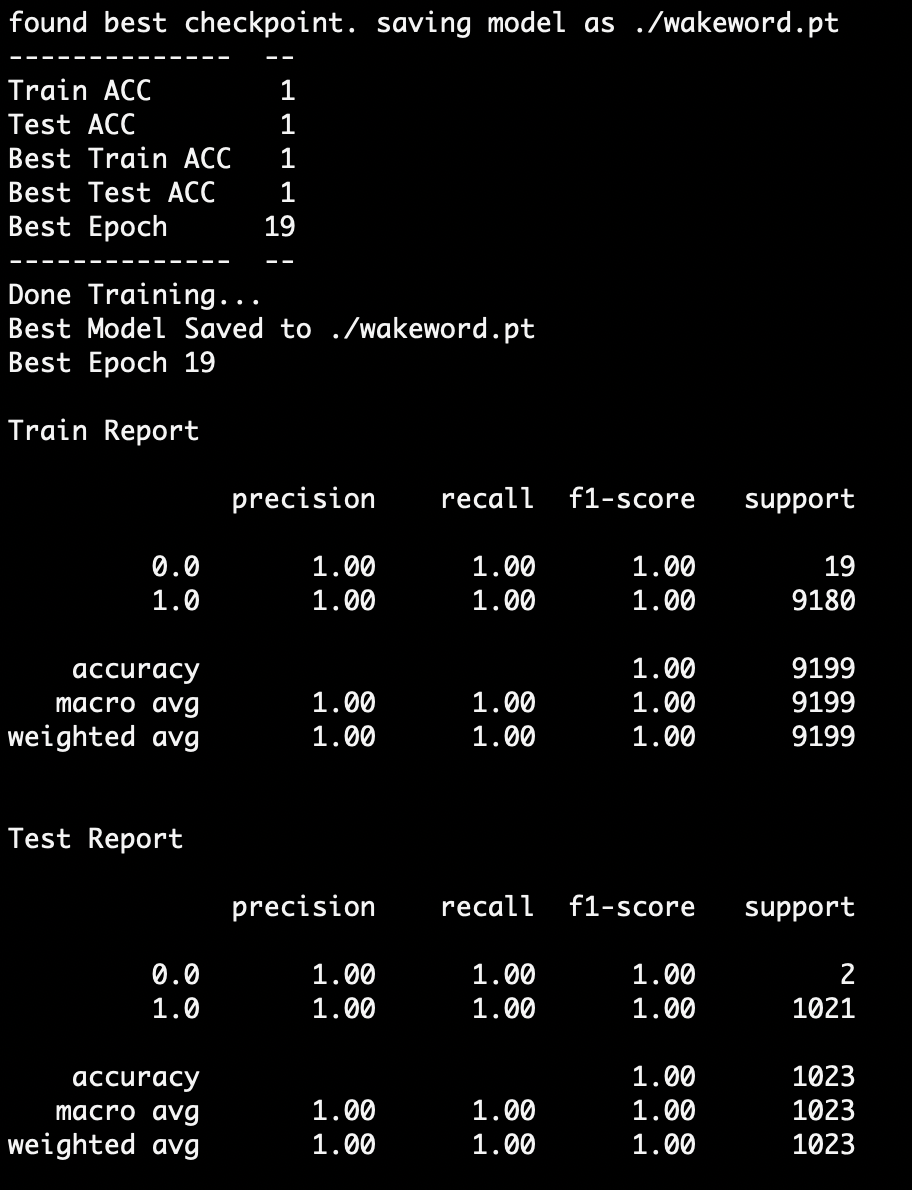
\includegraphics[width=\linewidth]{2.png}
    \caption{Accuracy2}
  \end{subfigure}
  \caption{Showing the accuracy of 20 epochs}
  \label{fig:accuracy}
\end{figure}

%------------------------------------------------
\section{Speech Recognition}
1. The model imports. We import the Wav2Vec2Tokenizer and Wav2Vec2ForCTC. The tokenizer is used for tokenization: converting the raw waveform into tokens that can be fed to the model; Wav2Vec2ForCTC represents the CTC-loss based model class.\\\\
2. Initializing the tokenizer. We use the facebook/wav2vec2-base-960h model for this. This model was pretrained on the LibriSpeech corpus and then finetuned on the 960 hours of data; hence the name.\\\\
3. Initializing the model. We use the same model for this purpose.\\\\
4. Read the sound file. Using librosa, we read the .wav file, with a sampling rate of 16000 Hz.\\\\
5. Tokenize the waveform. Using the tokenizer, we tokenize the waveform, and retrieve the input values.\\\\
6. Retrieve logits from the model. We retrieve logits from the model, reflecting the whole probability distribution over all possible output tokens.\\\\
7. Take the argmax value and decode into transcription. As with any logits, we can take argmax to find the most probable value(s) for the logits. We can batch decode these to find the text corresponding to the speech. Finally, we print this text.

%------------------------------------------------

\section{Restful apis}

1st api: to detect the record [speech recognition] based on Wave2Vec Bert \\
2nd api: to make string processing to process the text from the recording  \\
3rd api: to show the result add/remove a To-Do based on the text or do nothing

%------------------------------------------------
\section{UI}

We used the Flask template to show the record a voice and then based on that voice add/remove a todo    
%------------------------------------------------

\section{Docker}
We used docker to ship the system, we generated the dockers files to be compatible with Flask.

%----------------------------------------------------------------------------------------
%	REFERENCE LIST
%----------------------------------------------------------------------------------------

\begin{thebibliography}{9}


\bibitem{youtube} 
The A.I. Hacker - Michael Phi,
\\\texttt{https://www.youtube.com/watch?v=ob0p7G2QoHA\&list=PL5rWfvZIL-NpFXM9nFr15RmEEh4F4ePZW}

\bibitem{wav2vec} 
Patrick von Platen,
\\\texttt{https://huggingface.co/blog/fine-tune-wav2vec2-english}
\end{thebibliography}

\end{document}